
\section{Simplified geometry experiments with PISM}\label{sec:simp}

There have been three stages of ice sheet model intercomparisons based on simplified geometry experiments since the early 1990s \cite{BuelerSpray}.\index{EISMINT!defined}

EISMINT I \cite[ European Ice Sheet Modeling INiTiative]{EISMINT96}\footnote{See \url{http://homepages.vub.ac.be/\%7Ephuybrec/eismint.html}.} was the first of these and involved only the isothermal shallow ice approximation (SIA).  Both fixed margin and moving margin experiments were performed in EISMINT I, and various conclusions were drawn about the several numerical schemes used in the intercomparison.  EISMINT I is superceded, however, by verification using the full variety of known exact solutions to the isothermal SIA \cite{BLKCB}.  The ``rediscovery'', since EISMINT I, of the Halfar similarity solution with zero accumulation \cite{Halfar83}, and verification runs using that solution, already suffices to measure the isothermal SIA performance of PISM more precisely than would be allowed by comparison to EISMINT I results.

EISMINT II \cite{EISMINT00} pointed out interesting and surprising properties of the thermocoupled SIA.  References \cite{BBL,Hindmarsh04,Hindmarsh06,PayneBaldwin,SaitoEISMINT,BBssasliding} each interpret the EISMINT II experiments and/or describe attempts to add more complete physical models to ``fix'' the (perceived and real) shortfalls of ice sheet model behavior on EISMINT II experiments.  We believe that the discussion in \cite{PayneDongelmans,PayneBaldwin,BBL} adequately explains the ``spokes'' in EISMINT II experiment F as a genuine fluid instability, while \cite{Fowler01} and Appendix B of \cite{BBssasliding} adequately cautions against the continuum model that generates the ``spokes'' in EISMINT II experiment H.   Thus we can move on from that era of controversy.  In any case, PISM has built-in support for all of the published and unpublished EISMINT II experiments; these are described in the next subsection.

The ISMIP (Ice Sheet Model Intercomparison Project)\footnote{See \url{http://homepages.vub.ac.be/\%7Ephuybrec/ismip.html}.}\index{ISMIP!defined} round of intercomparisons covers 2008--2013 (at least).  There are four components of ISMIP substantially completed, namely HOM = Higher Order Models \cite{ISMIPHOM,HOMelmer}, HEINO = Heinrich Event INtercOmparison \cite{GreveTakahamaCalov,Calovetal2009HEINOfinal}, MISMIP (below), and MISMIP3d (also below).

PISM participated in HEINO, but this ability is unmaintained.   We believe\index{ISMIP!interpretation of HEINO results} the continuum problem described by HEINO, also used in EISMINT II experiment H (above), is not meaningfully approximate-able because of a required discontinuous jump in the basal velocity field.  The continuum problem predicts infinite vertical velocity because of this jump \cite[Appendix B]{BBssasliding}.  Details of the numerical schemes and their results are irrelevant if the continuum model makes such a prediction.  PISM offers the physical continuum model described in \cite{BBssasliding}, an SIA+SSA hybrid, as an alternative to the continuum model used in ISMIP-HEINO and EISMINT II experiment H.  Indeed the SIA+SSA hybrid is offered as a unified shallow model for real ice sheets (section \ref{sec:dynamics}).

There is no current plan to support ISMIP-HOM \cite{ISMIPHOM,HOMelmer}, but comparison of shallow PISM results to exact Stokes solutions is a goal for PISM evaluation.

A third and fourth ISMIP parts are the two parts of the Marine Ice Sheet Model Intercomparison Project, MISMIP\index{ISMIP!MISMIP} \cite{MISMIP2012} and MISMIP3D\index{ISMIP!MISMIP3d} \cite{MISMIP3d2013}.  These experiments are supported in PISM, as described in subsections \ref{subsect:MISMIP} and \ref{subsect:MISMIP3d} below.


\subsection{EISMINT II}\label{subsect:EISMINTII}
\optsection{EISMINT II}

There are seven experiments described in the published EISMINT II writeup \cite{EISMINT00}.\index{EISMINT}  They are named A, B, C, D, F, G, and H.  They have these common features:\begin{itemize}
\item runs are for 200,000 years, with no prescribed time step;
\item a $61\times 61$ horizontal grid on a square domain ($1500$ km side length) is prescribed;
\item surface inputs (temperature and mass balance) have angular symmetry around the grid center;
\item the bed is flat and does not move (no isostasy);
\item the temperature in the bedrock is not modeled;
\item only the cold (not polythermal) thermomechanically-coupled SIA is used \cite{EISMINT00}; and
\item basal melt rates do not affect the evolution of the ice sheet.
\end{itemize}
The experiments differ from each other in their various combinations of surface temperature and mass balance parameterizations.  Experiments H and G involve basal sliding, under the physically-dubious SIA sliding rubric \cite[Appendix B]{BBssasliding}, while the others don't.  Four experiments start with zero ice (A,F,G,H), while the other experiments (B,C,D) start from the final state of experiment A.

In addition to the seven experiments published in \cite{EISMINT00}, there were an additional five experiments described in the EISMINT II intercomparison description 
\cite{EISIIdescribe}, labeled E, I, J, K, and L.\index{EISMINT!unpublished additional EISMINT II experiments}  These experiments share most features listed above, but with the following differences.  Experiment E is the same as experiment A except that the peak of the accumulation, and also the low point of the surface temperature, are shifted by 100 km in both $x$ and $y$ directions; also experiment E starts with the final state of experiment A.  Experiments I and J are similar to experiment A but with non-flat ``trough'' bed topography.  Experiments K and L are similar to experiment C but with non-flat ``mound'' bed topography.

See table \ref{tab:eisII} for how to run all EISMINT II experiments in PISM.  Note that the vertical grid is not specified in EISMINT II, but it seems that good simulation of the thermomechanically-coupled conditions near the base of the ice requires relatively-fine resolution there.  (It is difficult to be quantitative because of a lack of theory.)  We suggest using the default unequally-spaced grid with 61 levels, which gives a grid spacing of 18 m in the ice layer closest to the bed.  Alternatively these experiments can be done with an equally-spaced grid; in this case we suggest using 201 vertical levels to give 20 m spacing, for example.

These SIA-only simulations parallelize well.  Very roughly, for the standard $61\times 61$ horizontal grid, wall-clock-time speedups will occur up to about 30 processors.  Runs on finer (horizontal) grids will benefit from even more processors.

Table \ref{tab:eisII} shows how all EISMINT II experiments are done in PISM.  Experiments below the horizontal line in Table \ref{tab:eisII} are only documented in \cite{EISIIdescribe}.

\begin{table}[ht]
\centering
\small
\begin{tabular}{@{}llll}\toprule
\textbf{Command: ``\texttt{pisms }'' $+$} & \textbf{Relation to experiment A} \\
\midrule
\texttt{-eisII A -Mx 61 -My 61 -Mz 61 -y 200000 -o eisIIA.nc} & \\
\texttt{-eisII B -i eisIIA.nc -y 2e5 -o eisIIB.nc} & warmer \\
\texttt{-eisII C -i eisIIA.nc -y 2e5 -o eisIIC.nc} & less snow (lower accumulation)\\
\texttt{-eisII D -i eisIIA.nc -y 2e5 -o eisIID.nc} & smaller area of accumulation \\
\texttt{-eisII F -Mx 61 -My 61 -Mz 61 -y 2e5 -o eisIIF.nc} & colder; famous spokes \cite{BBL} \\
\texttt{-eisII G -Mx 61 -My 61 -Mz 201 -y 2e5 -o eisIIG.nc} & sliding (regardless of temperature) \\
\texttt{-eisII H -Mx 61 -My 61 -Mz 201 -y 2e5 -o eisIIH.nc} & melt-temperature activated sliding \\ \midrule
\texttt{-eisII E -i eisIIA.nc -y 2e5 -o eisIIE.nc} & shifted climate maps \\
\texttt{-eisII I -Mx 61 -My 61 -Mz 201 -y 2e5 -o eisIII.nc} & trough topography \\
\texttt{-eisII J -i eisIII.nc -y 2e5 -o eisIIJ.nc} & trough topography and less snow \\
\texttt{-eisII K -Mx 61 -My 61 -Mz 201 -y 2e5 -o eisIIK.nc} & mound topography \\
\texttt{-eisII L -i eisIIK.nc -y 2e5 -o eisIIL.nc} & mound topography and less snow \\
\bottomrule
\normalsize
\end{tabular}
\caption{Running the EISMINT II experiments in PISM.\index{PISM!running the EISMINT II experiments in}  Use \texttt{-skip -skip_max 5}, on the $61\times 61$ default grid, for significant speedup.}
\label{tab:eisII}
\end{table}

The EISMINT II experiments can be run with various modifications of the default settings.  Of course the grid can be refined.  For instance, a twice as fine grid in the horizontal is ``\texttt{-Mx 121 -My 121}''.  Table \ref{tab:eisIIoptions} lists some optional settings which are particular to the EISMINT II experiments.

\begin{table}[ht]
\centering
\small
\begin{tabular}{@{}lllp{0.45\linewidth}}\toprule
\textbf{Option} & \textbf{Default values [expers]} & \textbf{Units} & \textbf{Meaning} \\\midrule
\intextoption{eisII} & A & &  Choose single character name of EISMINT II \cite{EISMINT00} simplified geometry experiment.  See Table \ref{tab:eisII}. \\
\intextoption{Mmax} & 0.5 [ABDEFGHIK], 0.25 [CJL] & m$/$a & max value of accumulation rate \\
\intextoption{Rel} & 450 [ABEFGHIK], 425 [CDJL] & km & radial distance to equilibrium line \\
\intextoption{Sb} & $10^{-2}$ [\emph{all}] & (m/a)/km & radial gradient of accumulation rate \\
\intextoption{ST} & $1.67 \times 10^{-2}$ [\emph{all}] & K/km & radial gradient of surface temperature\\
\intextoption{Tmin} & 238.15 [ACDEGHIJKL], & K & max of surface temperature \\
 & 243.15[B], 223.15[F] & & \\
\intextoption{bmr_in_cont} & & & Include the basal melt rate in the mass continuity computation; overrides EISMINT II default. \\
\bottomrule\normalsize
\end{tabular}
\caption{Changing the default settings for EISMINT II}
\label{tab:eisIIoptions}
\end{table}

In PISM the height of the computational box, the quantity set by \texttt{-Lz}, is set at the beginning of the run.  It is chosen for the EISMINT II experiments according to the observed maximum values occuring in standard runs.  If the ice thickens beyond the chosen level for the top of the computational box then additional layers are automatically added to the computational grid.  In fact, if the ice grows above the height of the computational box then a message appears, \texttt{PISM WARNING: max ice thickness ... is greater than the height of the computational box ...}, and then at least two additional levels are added to the vertical grid.  However, in general this mechanism can run away to use up all memory in extreme cases so, if the height of the computational box grows so large that the grid has more than twice the original number of vertical levels, then PISM produces an error message and stops.   Therefore it is possible that the number of vertical levels at the end of the run exceeds the initial \texttt{-Mz} value.  Setting EISMINT II options \texttt{-Mmax} or \texttt{-Sb} to produce higher accumulation rates than the default values (see table \ref{tab:eisIIoptions}) may cause the ice sheet to thicken above the standard thickness and therefore trigger this automatic extension mechanism.  Similarly, colder ice caused by nonstandard \texttt{-Tmin} or \texttt{-ST} values can produce unusually thick ice.  The user may always choose to use a larger, more conservative value for option \texttt{-Lz}, however.

See subdirectory \verb|examples/eismintII/| for a simple helper script \verb|runexp.sh|.


\subsection{MISMIP}\label{subsect:MISMIP}
\optsection{MISMIP}\index{ISMIP!MISMIP}

This intercomparison addresses grounding line dynamics by considering an idealized one-dimensional stream-shelf system.  In summary, a flowline ice stream and ice shelf system is modeled, the reversibility of grounding line movement under changes in the ice softness is tested, different sliding laws are tested, and the behavior of grounding lines on reverse-slope beds is tested.  The intercomparison process is described at the website

\centerline{\url{http://homepages.ulb.ac.be/~fpattyn/mismip/}}

\noindent Find a full text description there, along with the published report on the results \cite{MISMIP2012}; that paper includes results from PISM version 0.1.  These documents are essential reading for understanding MISMIP results generally, and for appreciating many of the comments in this subsection.

PISM's version of MISMIP includes an attached ice shelf even though modeling the shelf is theoretically unnecessary in the MISMIP flow line case.  The analysis in \cite{SchoofMarine1} shows that the only effect of an ice shelf, in the flow line case, is to transfer the force imbalance at the calving front directly to the ice column at the grounding line.  (Such an analysis does not apply to ice shelves with two horizontal dimensions; real ice shelves have ``buttressing'' and ``side drag'' and other forces not present in the flow line \cite{Goldbergetal2009}.  See the Ross ice shelf example in section \ref{sec:ross}, for example.)

We use the usual PISM ice shelf model, with two horizontal dimensions, to do MISMIP.  We must adapt it to do a flow line problem (see section \ref{sec:flowline-modeling}).  The flow direction for MISMIP is taken to be ``$x$''.  We periodize the cross-flow direction ``$y$'', and use the minimum number of points in the $y$-direction which maintains function.  This number turns out to be ``\texttt{-My 3}''; fewer points than this in the cross-flow direction confuses the finite difference scheme.

PISM has can do MISMIP experiments with either of two applicable ice dynamics models.  Model 1 is a pure SSA model; ``category 2'' in the MISMIP classification.  Model 2 combines SIA and SSA velocities as described in \cite{Winkelmannetal2011}; ``category 3'' because it resolves ``vertical'' shear (i.e.~using SIA flow).

Note there are many runs for a complete MISMIP intercomparison submission.  Specifically, for a given model there are $62$ runs for each grid choice, and three (suggested) grid choices, so a full suite is $3 \times 62 = 186$ runs.

The coarsest grid (``mode 1'') has 12 km spacing.  The finest grid, ``mode 2'' with 1.2 km spacing, accounts for all the compute time, however; in the MISMIP description it is 1500 grid spaces in the flow line direction (= 3001 grid \emph{points} in PISM's doubled computational domain), a very fine grid which imposes severe time-step restrictions on the explicit methods in PISM.  In between is ``mode 3'', a mode interpretable by the intercomparison participant, and here we just use a 6 km grid.

The implementation of MISMIP in PISM conforms fairly-closely to the intercomparison description.  However, that document specifies
\begin{quotation}
\dots we require that the rate of change of grounding line position be $0.1$ m/a or less, while the rate of change of ice thickness at each grid point at which ice thickness is defined must be less than $10^{-4}$ m/a \dots
\end{quotation}
as a standard for ``steady state''. PISM does not include a stopping criterion such as ones described here. However, we report enough information, in PISM output files with scalar and spatially-variable time-series, to compute a grounding line rate or the time at which the thickness rate of change drops below $10^{-4}$ m/a.

See

  \centerline{\texttt{examples/mismip/mismip2d/README.md}}

\noindent for usage of the scripts that run MISMIP experiments in PISM.  For example, as described in this \texttt{README.md}, the commands

\begin{verbatim}
$ ./run.py -e 1a --mode=1 > experiment-1a-mode-1.sh
$ bash experiment-1a-mode-1.sh 2 >& out.1a-mode-1 &
$ ./plot.py ABC1_1a_M1_A7.nc -p -o profileA7.png
\end{verbatim}

\noindent first generate a bash script, then use it to do a run which takes about 20 minutes, and then generate an image in \texttt{.png} format.  Note that step 7 is in the middle of the experiment.  It is shown in Figure \ref{fig:MISMIPmodel1exper1aA7} (left).
 
\begin{figure}[ht]
\centering
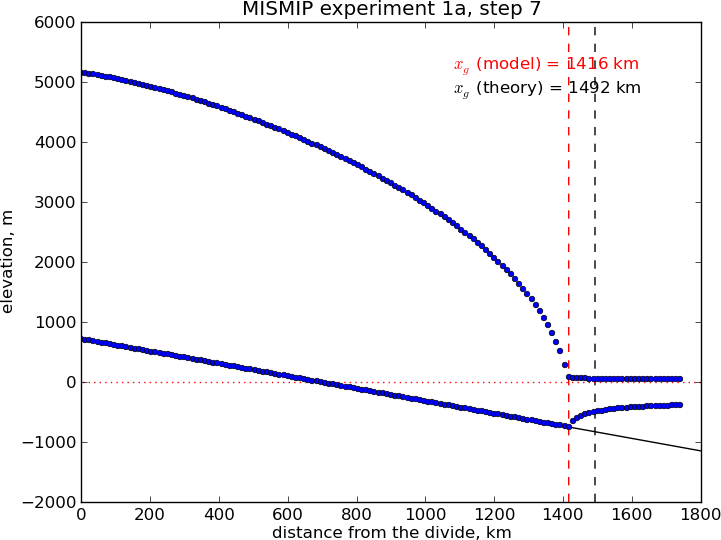
\includegraphics[width=3.3in,keepaspectratio=true]{profileA7} \,
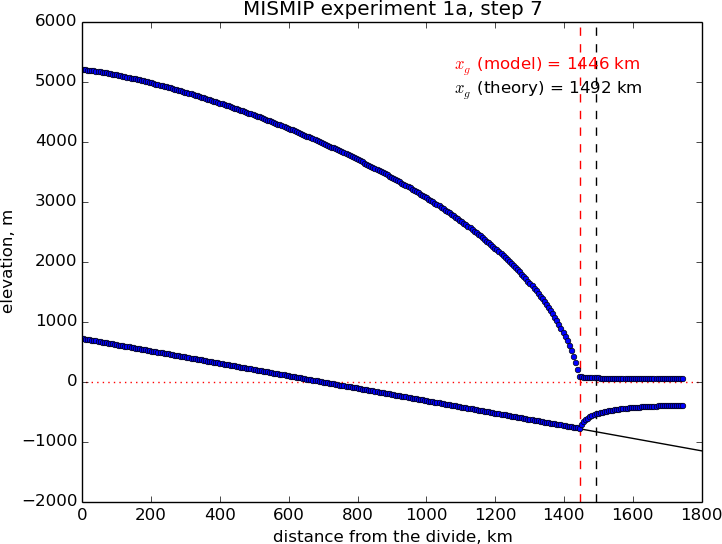
\includegraphics[width=3.3in,keepaspectratio=true]{profileA7-M3}
\caption{A marine ice sheet profile in the MISMIP intercomparison; PISM model 1, experiment 1a, at step 7.  Left: grid mode 1 (12 km grid).  Right: grid mode 3 (6 km grid).}
\label{fig:MISMIPmodel1exper1aA7}
\end{figure}

\begin{figure}[ht]
\centering
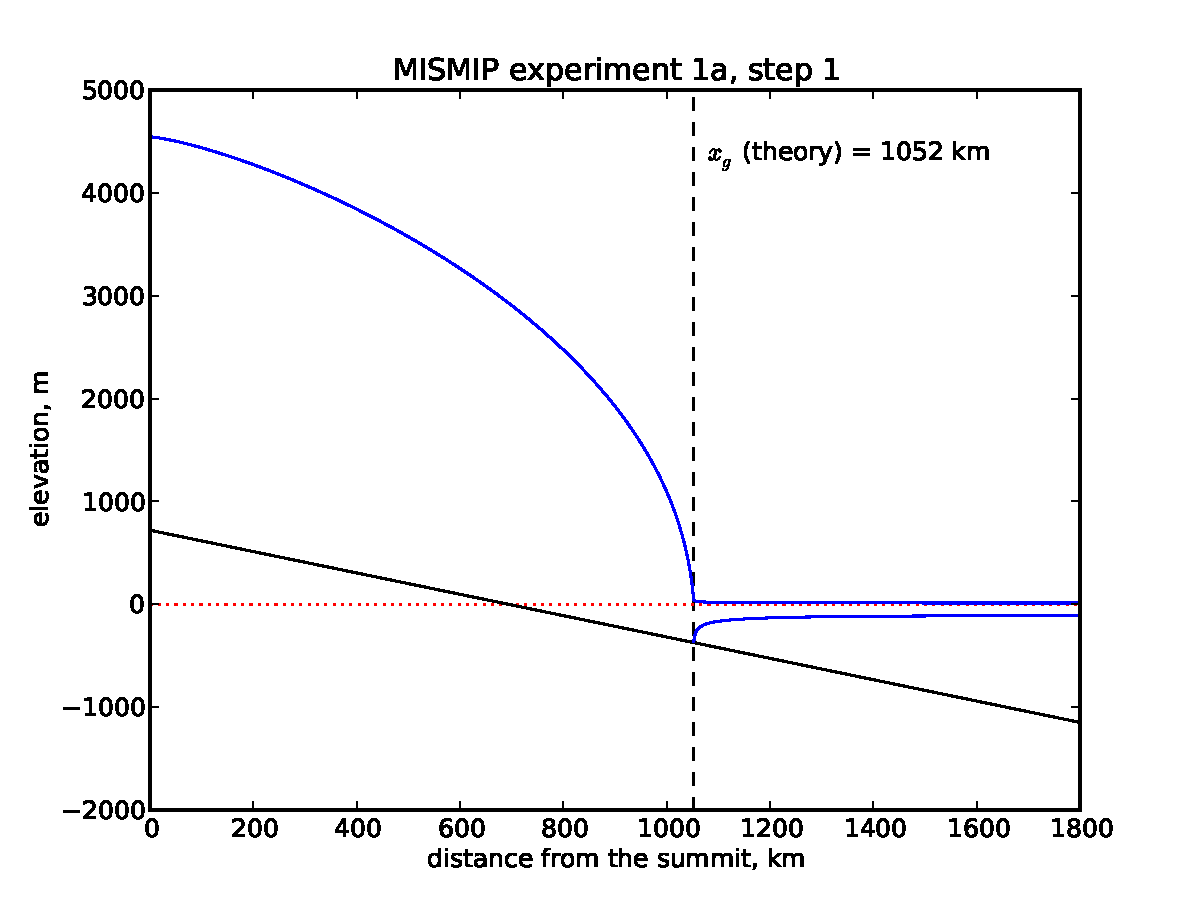
\includegraphics[width=4.0in,keepaspectratio=true]{SM-1a-A1}
\caption{Analytical profile for steady state of experiment 1a, step 1, from theory in \cite{SchoofMarine1}.  This is a boundary layer asymptotic matching result, but not the exact solution to the equations.}
\label{fig:SMexper1aM1A1}
\end{figure}

The script \texttt{MISMIP.py} in \texttt{examples/mismip/mismip2d} has the ability to compute the profile from the Schoof's \cite{SchoofMarine1} asymptotic-matching boundary layer theory.  This script is a Python translation, using \texttt{scipy} and \texttt{pylab}, of the \Matlab codes in \url{http://homepages.ulb.ac.be/~fpattyn/mismip/MISMIP_distribution.tar}.  For example,

\begin{verbatim}
$ python MISMIP.py -o mismip_analytic.png
\end{verbatim}
 
\noindent produces a \verb|.png| image file with Figure \ref{fig:SMexper1aM1A1}.

Generally the PISM result does not put the grounding line in the same location as Schoof's boundary layer theory, and at least at coarser resolutions the problem is with PISM's numerical solution, not with Schoof's semi-analytic theory.  Evidence that the problem is numerical can be found by looking at the ice flux.  Examining the diagnostic variable \texttt{cflx} (flux magnitude) in \texttt{ABC1_1a_M1_A1.nc} we see Figure \ref{fig:cflx1aA1} (left).  The flux should be a linear function because, at steady state, the flux $\bq$ solves $a=\Div\bq$ where $a$ is the constant (at least in MISMIP) surface mass balance, so at steady state $|\bq| = a x$, a line.

\begin{figure}[ht]
\centering
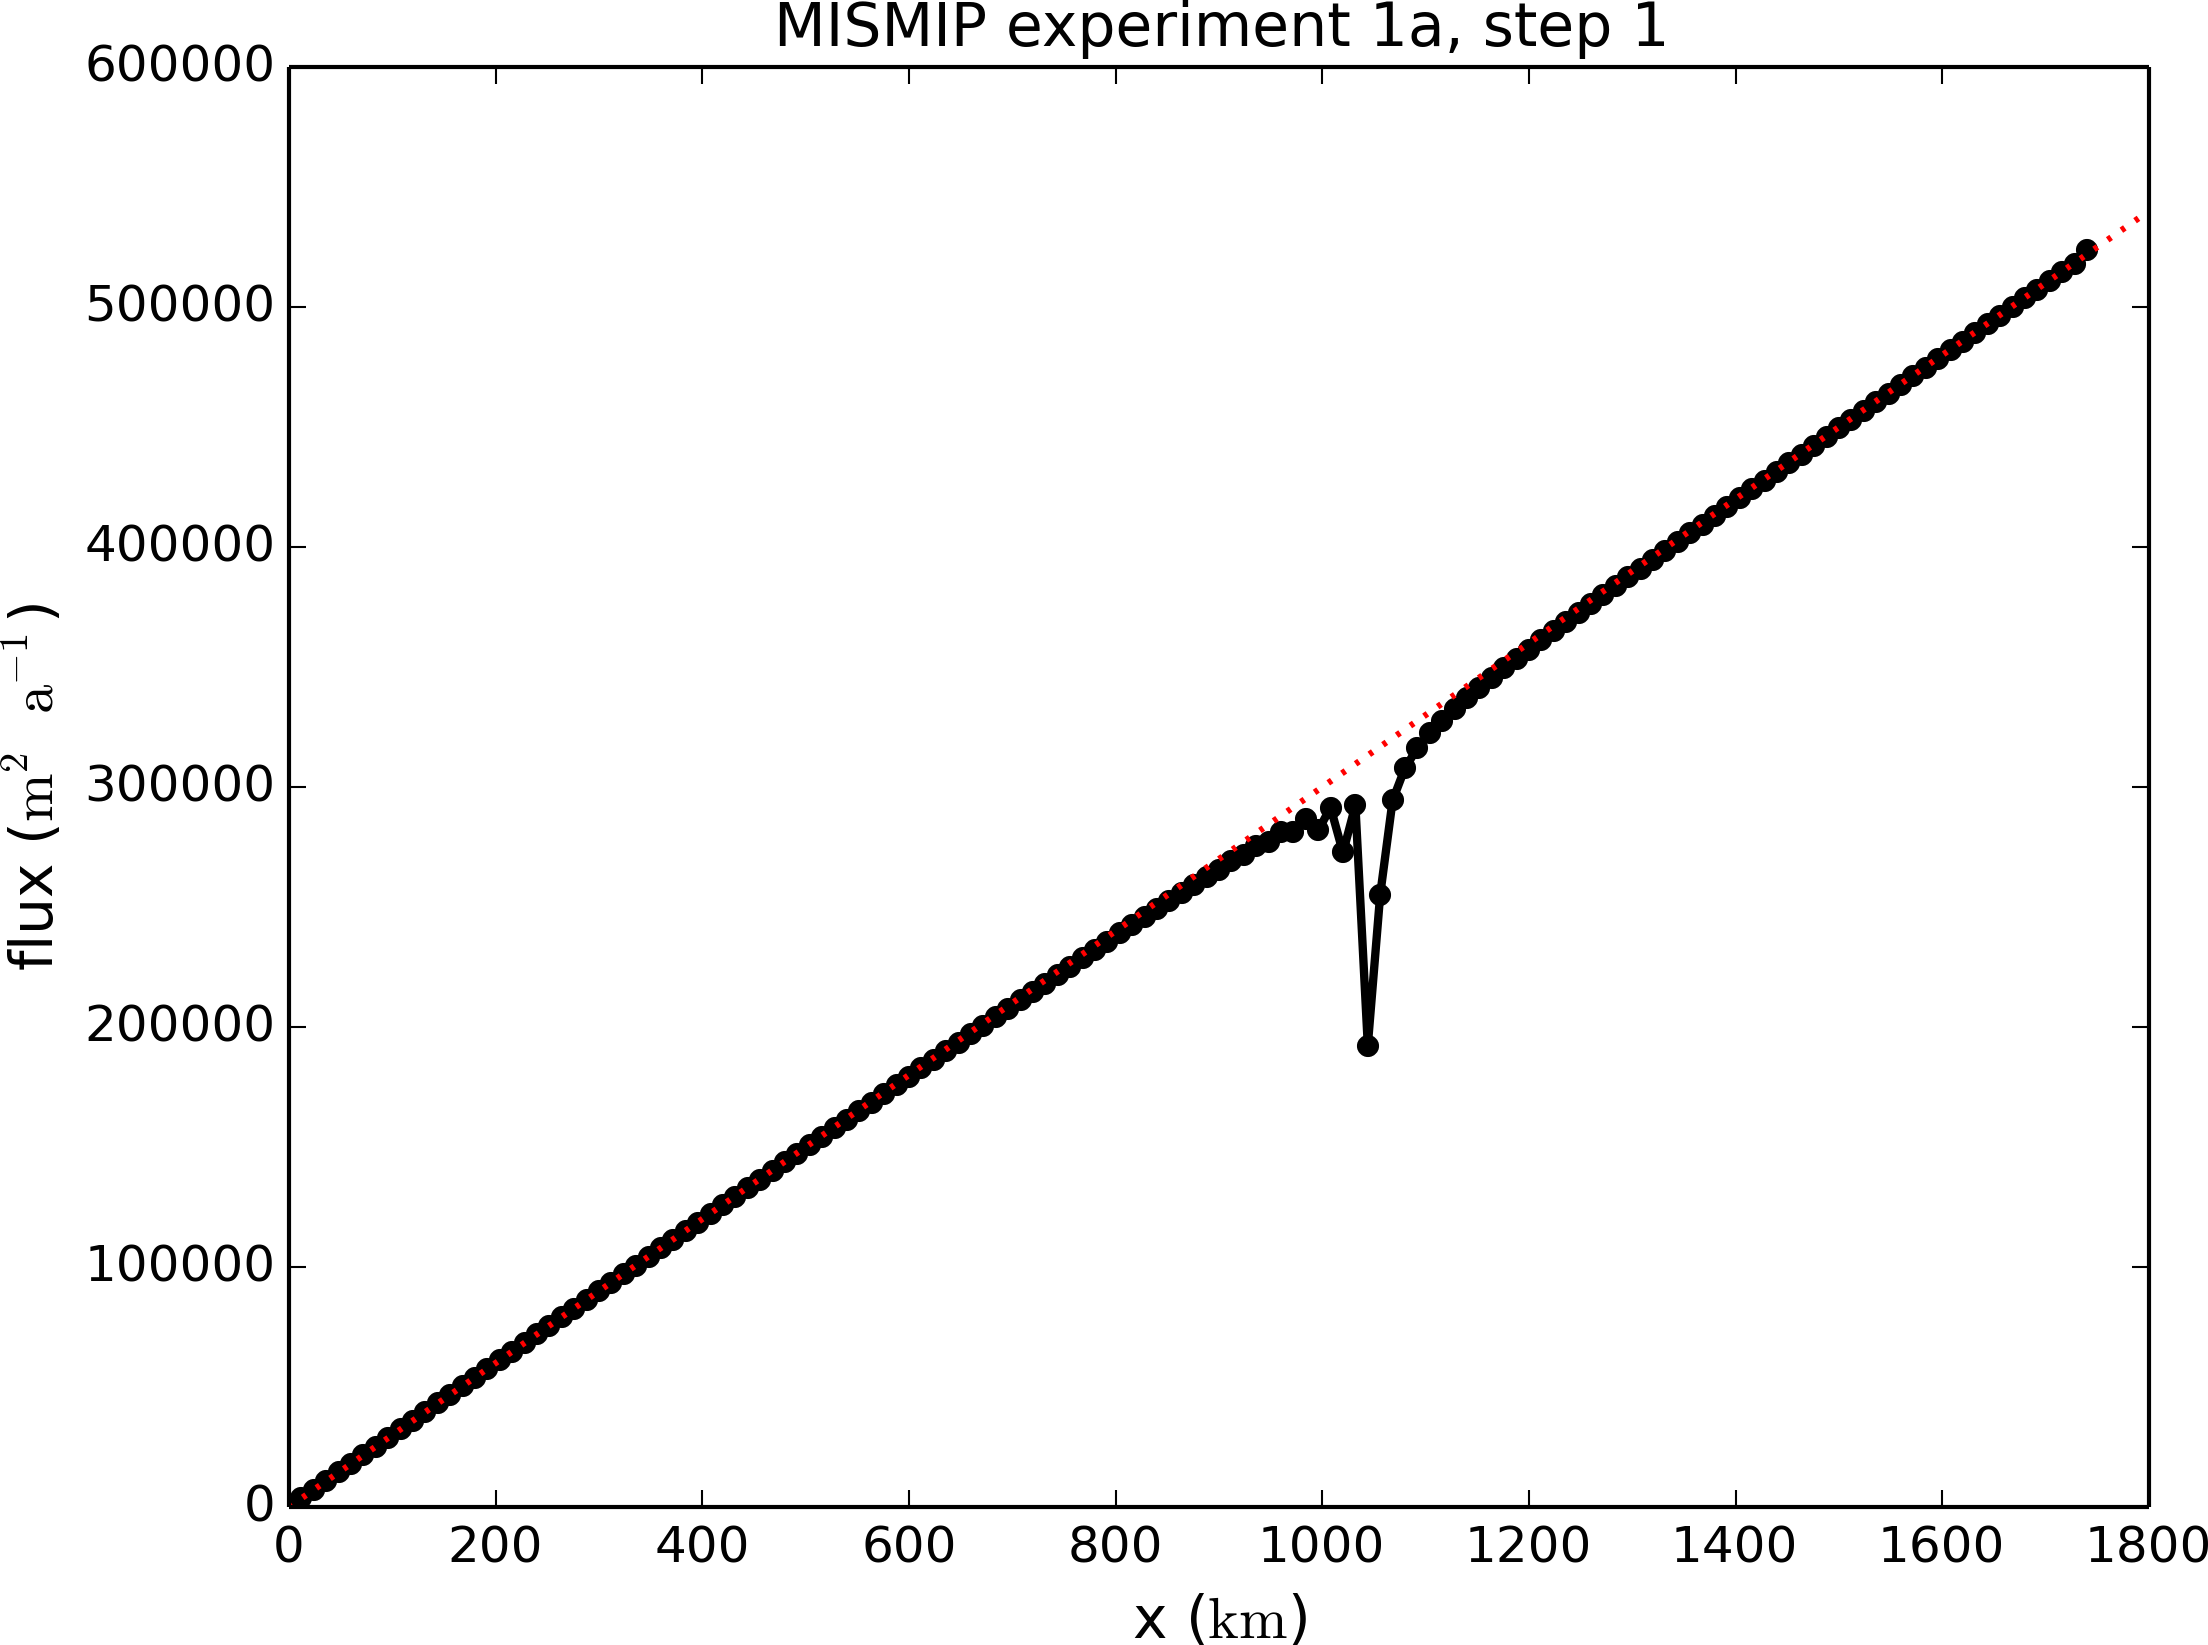
\includegraphics[width=3.3in,keepaspectratio=true]{fluxA1-M1} \,
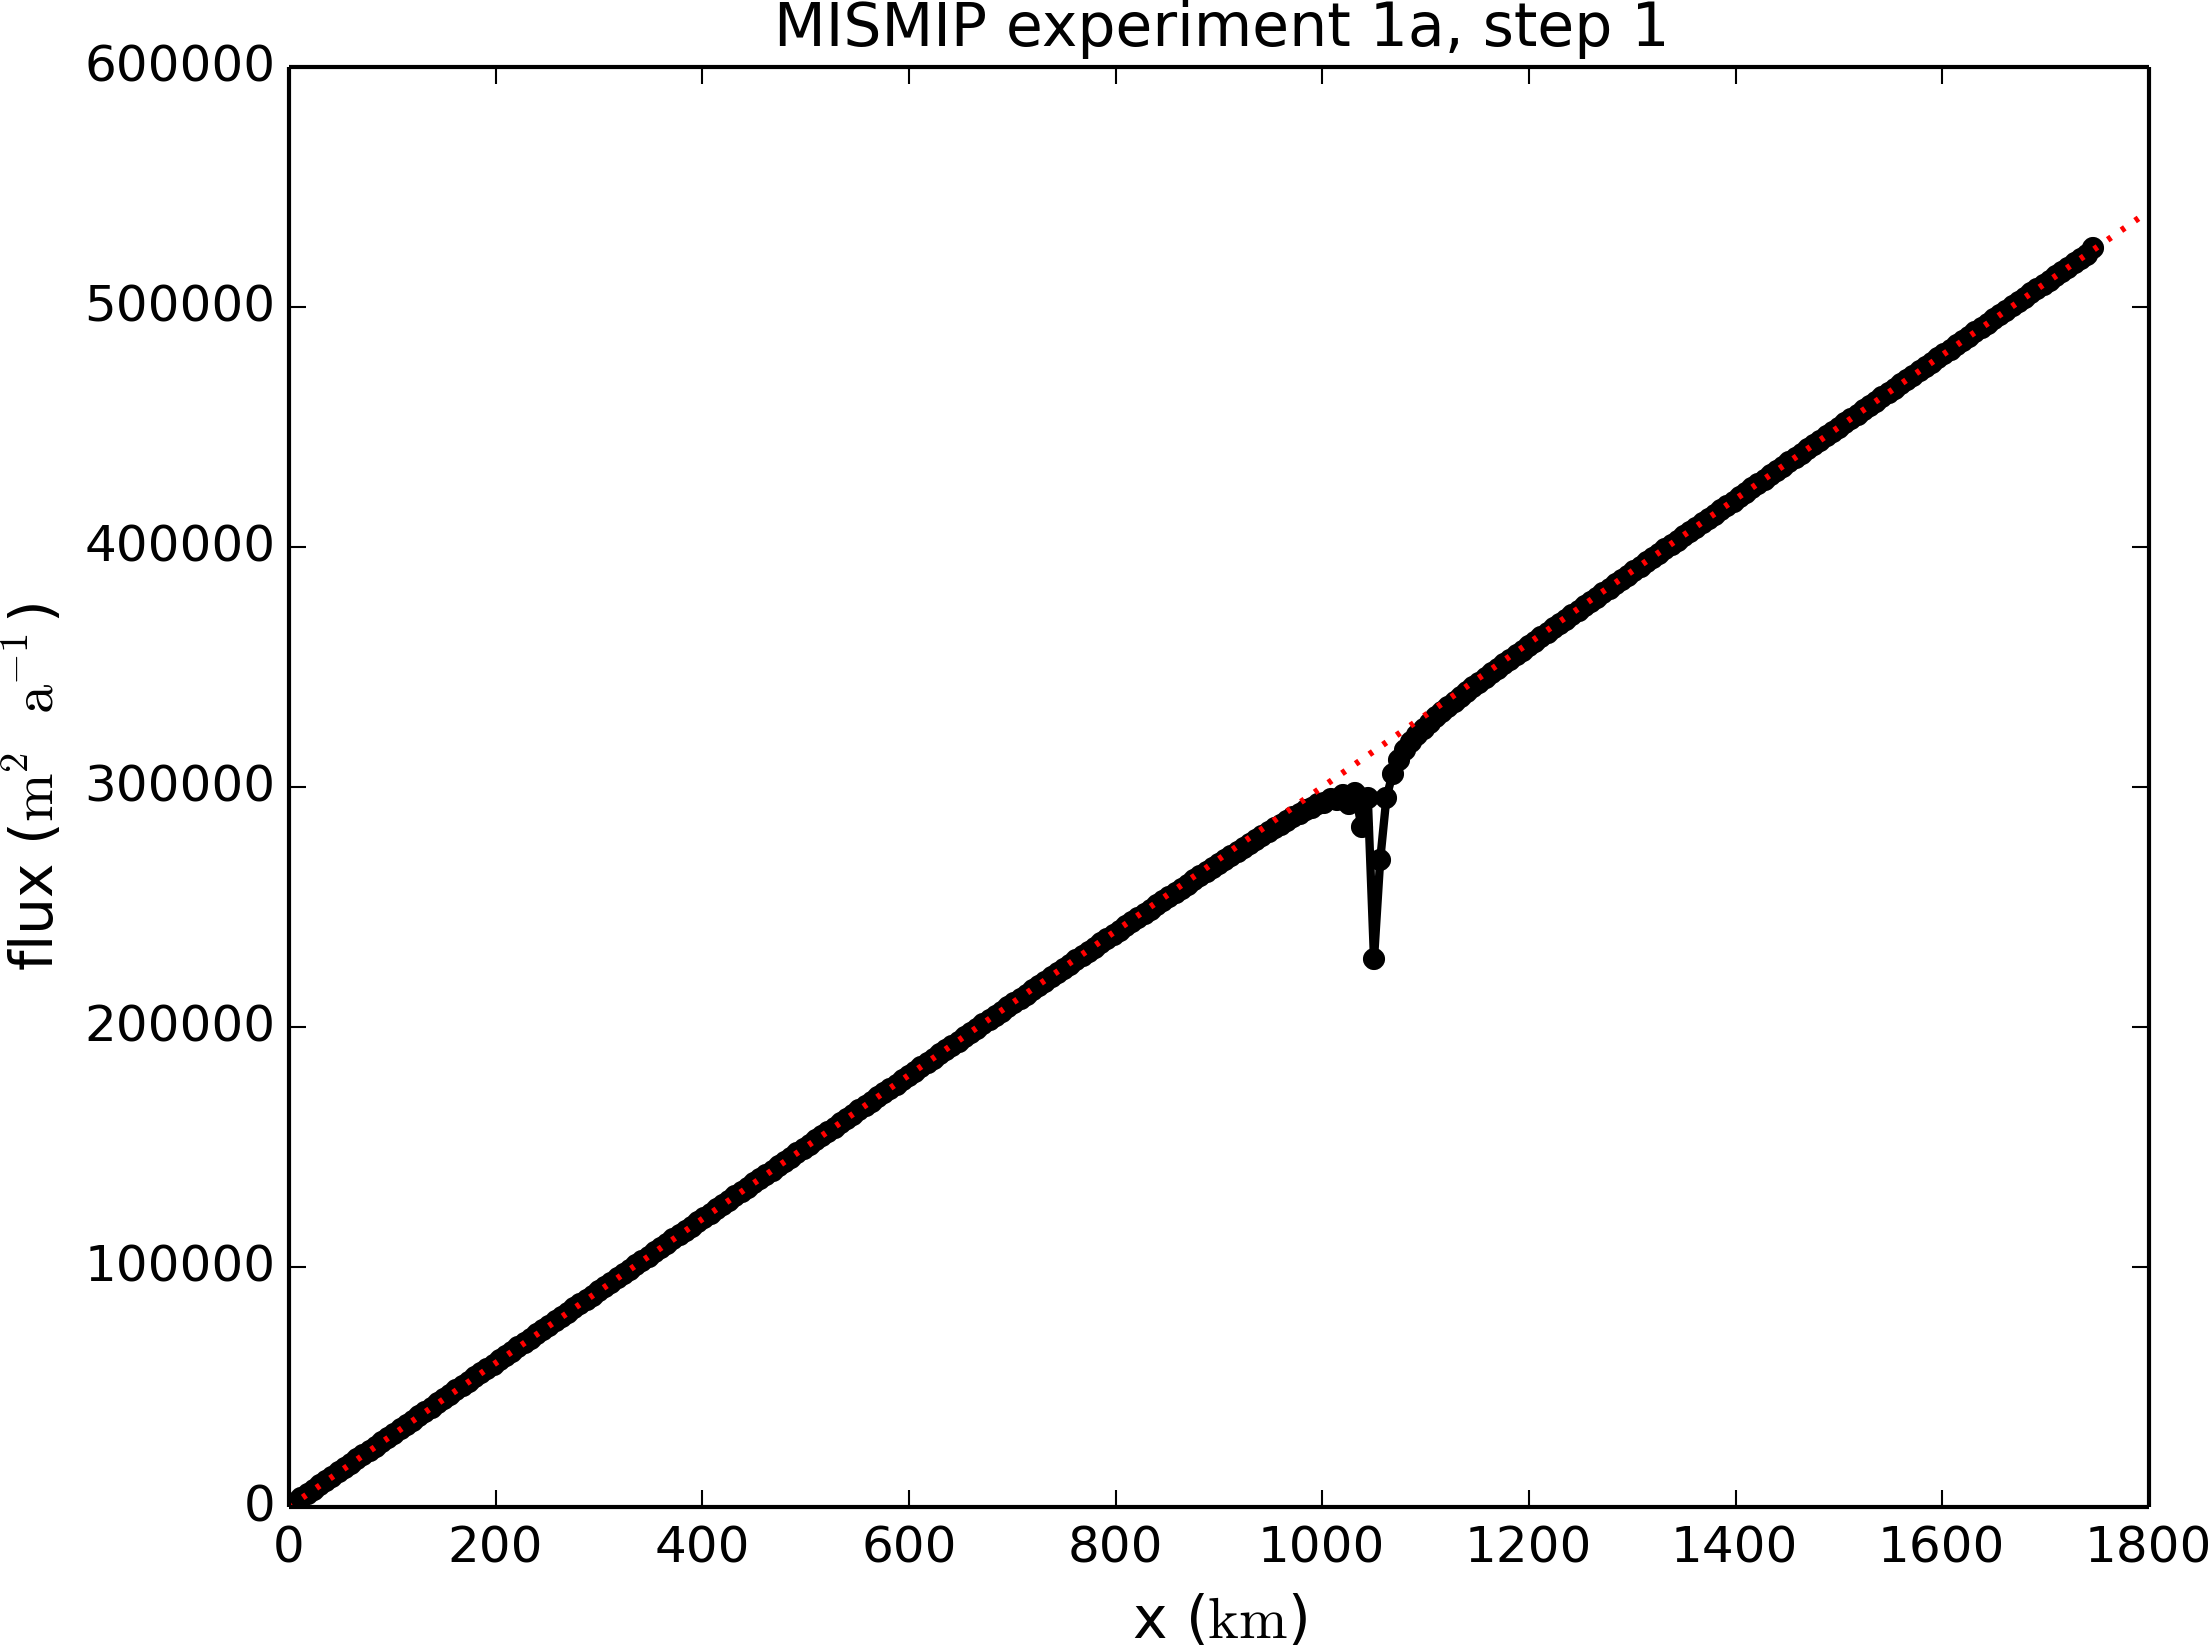
\includegraphics[width=3.3in,keepaspectratio=true]{fluxA1-M3}
\caption{Numerically-computed flux $\bq = \bar\bU\, H$, where $\bar\bU$ is the vertically-averaged horizontal velocity and $H$ the thickness, for steady state of experiment 1a, step 1.  Illustrates a significant numerical problem; it should be the dotted line, which has slope $a = 0.3$ m/a.  Left: grid mode 1.  Right: grid mode 3.}
\label{fig:cflx1aA1}
\end{figure}

By default \texttt{run.py} uses the asymptotic-matching thickness result from the \cite{SchoofMarine1} theory to initialize the initial ice thickness, as allowed by the MISMIP specification.

\begin{figure}[ht]
\centering
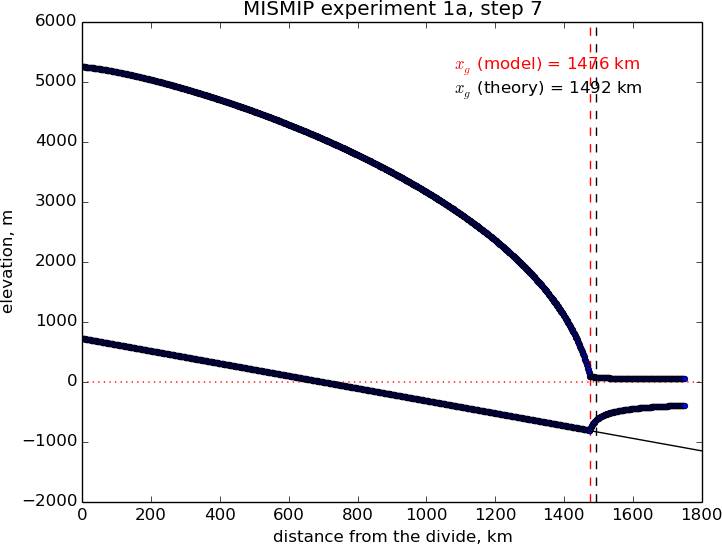
\includegraphics[width=3.3in,keepaspectratio=true]{profileA7-M2} \,
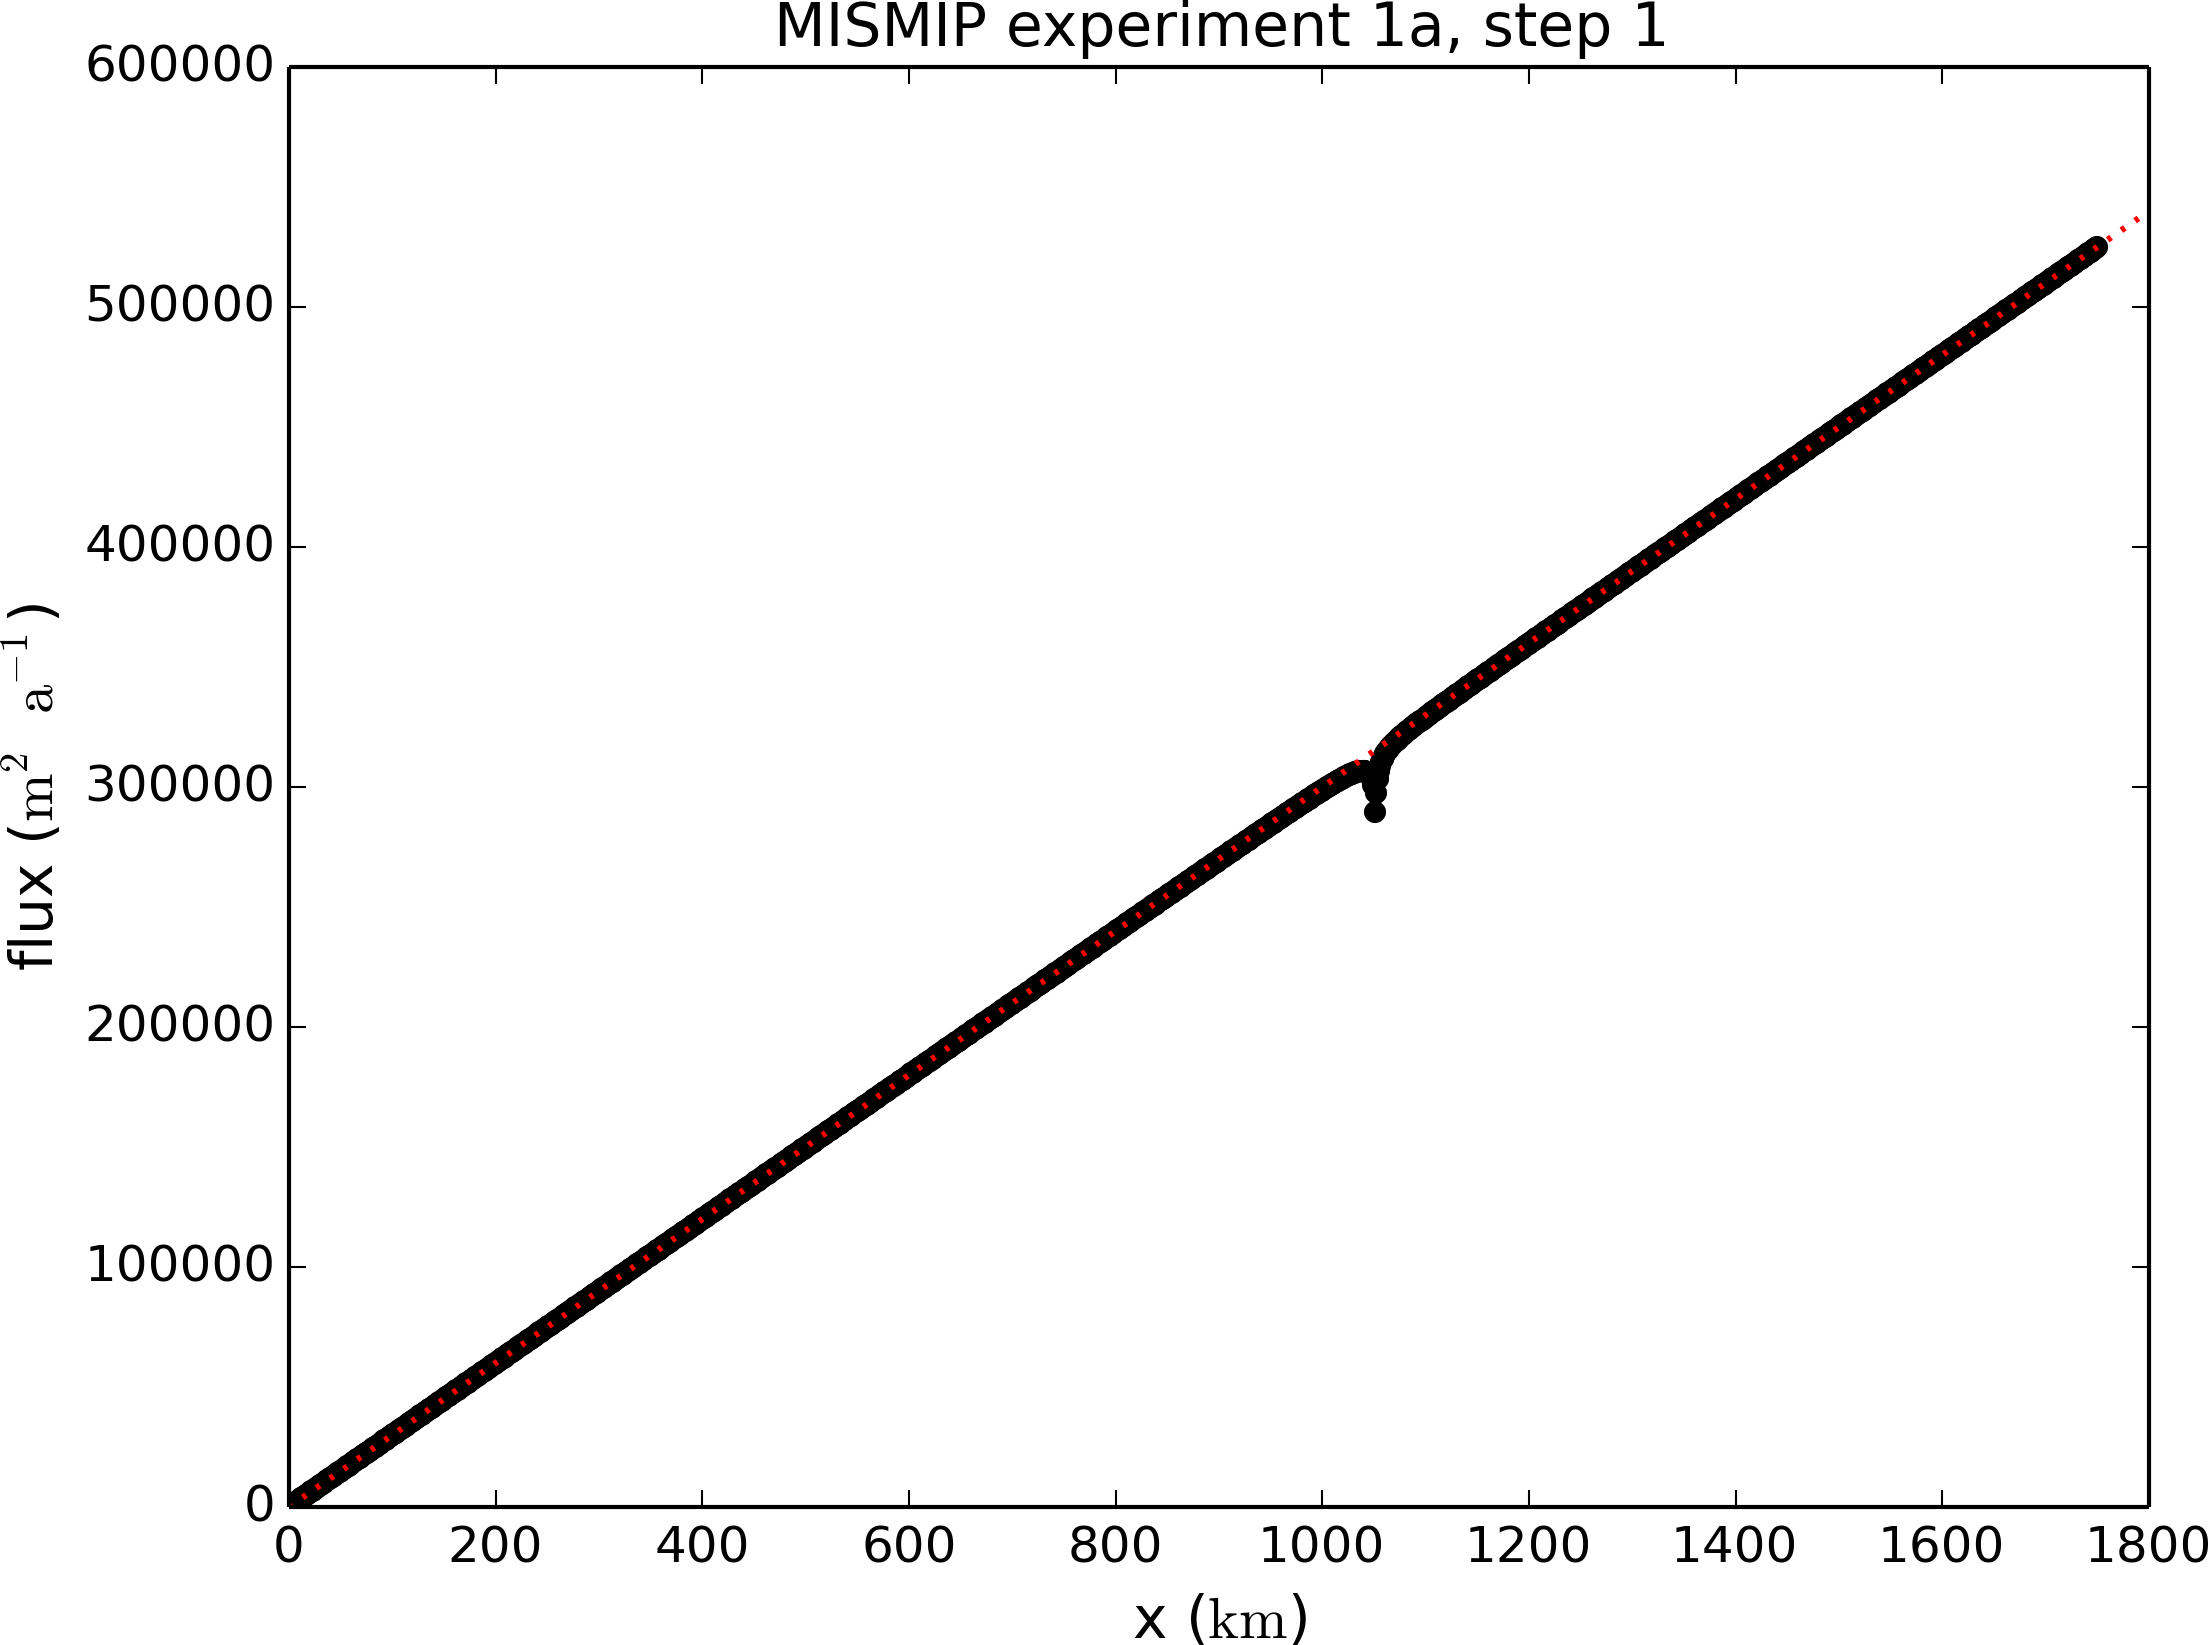
\includegraphics[width=3.3in,keepaspectratio=true]{fluxA1-M2}
\caption{Results from grid mode 2, with 1.2 km spacing, for steady state of experiment 1a.  Left: profile at step 7 (compare Figure \ref{fig:MISMIPmodel1exper1aA7}).  Right: numerically-computed flux at step 1 (compare Figure \ref{fig:cflx1aA1})}
\label{fig:MISMIPmode2results}
\end{figure}

The effect when we do this at higher resolution is an improvement.  Results from grid mode 3 with 6 km spacing, instead of 12 km in mode 1, are in the right parts of Figure \ref{fig:MISMIPmodel1exper1aA7} and \ref{fig:cflx1aA1}.  The corresponding results from grid mode 2, with 1.2 km spacing, are in Figure \ref{fig:MISMIPmode2results}.  Note that the difference between the numerical grounding line location and the semi-analytical location has been reduced from 76 km for grid mode 1 to 16 km for grid mode 2 (a factor of about 5), by using a grid refinement from 12 km to 1.2 km (a factor of about 10).


\subsection{MISMIP3d}\label{subsect:MISMIP3d}
\optsection{MISMIP3d}\index{ISMIP!MISMIP3d}
The ice2sea MISMIP3d intercomparison is a two-horizontal-dimensional extension of the flowline case described above.  As before, in MISMIP3d the grounding line position and its reversibility under changes of physical parameters is analyzed.  Instead of changing the ice softness, however, the spatial distribution and magnitude of basal friction is adjusted between experiments.  The applied basal friction perturbation of the basal friction is a localized gaussian ``bump'' and thus a curved grounding line is obtained.  In contrast to the flowline experiments, no (semi-)analytical solutions are available to compare to the numerical results.

A full description of the MISMIP3d experiments can be found at

\centerline{\url{http://homepages.ulb.ac.be/~fpattyn/mismip3d/}}

\noindent and the results are published in \cite{MISMIP3d2013}.

A complete set of MISMIP3d experiments consists of three runs: Firstly, a flowline solution on a linearly-sloped bed, similar to the flowline MISMIP experiments of the previous section, is run into a steady state (``standard experiment \texttt{Stnd}'').  Then the localized sliding perturbation is applied (``perturbation experiment'')  causing the grounding line to shift and lose symmetry.  Two different amplitudes of the perturbation are considered (``\texttt{P10}'' and ``\texttt{P75}'').  Finally, beginning from the final state of the perturbation experiment, the sliding perturbation is removed and the system is run again into steady state (``reversibility experiment'').  The resulting geometry, in particular the grounding line position, is expected to be close to that of the standard experiment.  Expecting such reversibility assumes that a particular stationary ice geometry only depends on its physical parameters and boundary conditions and not on how it is dynamically reached.

For these experiments in PISM, a Python script generates a shell script which has the commands and options for running a MISMIP3d experiment.  The python script is \texttt{createscript.py} in the folder \texttt{examples/mismip/mismip3d/}.  Run

\begin{verbatim}
$ ./createscript.py -h
\end{verbatim}

\noindent to see a usage message.  A \texttt{README.md} gives a tutorial on how to use \texttt{createscript.py} and do the runs themselves.

For the flowline \texttt{Stnd} experiment, as in the MISMIP case, a computational domain with three grid points in the direction orthogonal to the ice flow (arbitrarily chosen as y-direction) is chosen by \texttt{createscript.py}.  For the perturbation and reversibility experiments a domain is defined which is symmetric along the ice-divide (mirror symmetry) and along the center line of the ice flow, while the side boundaries are periodic, which corresponds to a free-slip condition for the flow in x-direction. Though this choice of the symmetric computational domain increases computational cost, it allows us to use standard PISM without fixing certain boundary conditions in the code.  (That is, it avoids the issues addressed in the regional mode of PISM; see section \ref{sec:jako}.)

PISM participated in the MISMIP3d intercomparison project \cite{MISMIP3d2013} using version pism0.5, and the exact results can be reproduced using that version.  PISM's results, and the role of resolution and the new subgrid grounding line interpolation scheme are discussed in \cite{Feldmannetal2014}.

We observed a considerable improvement of the results with respect to the absolute grounding line positions compared to other models (e.g. the FE reference model Elmer/Ice) and to the reversibility when applying the subgrid grounding line interpolation method; see Figure \ref{fig:Subgl}.  Furthermore, we observed that only using SSA yields almost the same results as the full hybrid SIA+SSA computation for the MISMIP3D (and also the MISMIP) experiments, but, when not applying the SIA computation, after a considerably shorter computation time (about 10 times shorter).  We explain the small and almost negligible SIA velocities for the MISMIP(3D) experiments with the comparably small ice surface gradients in the MISMIP3d ice geometries.  See Fig.~\ref{fig:compSIASSA} for a comparison of SSA and SIA velocities in the MISMIP3D geometry.  Note that both Figures \ref{fig:Subgl} and \ref{fig:compSIASSA} were generated with resolution of $\Delta x = \Delta y = 1\;$km.

\begin{figure}[ht]
\centering
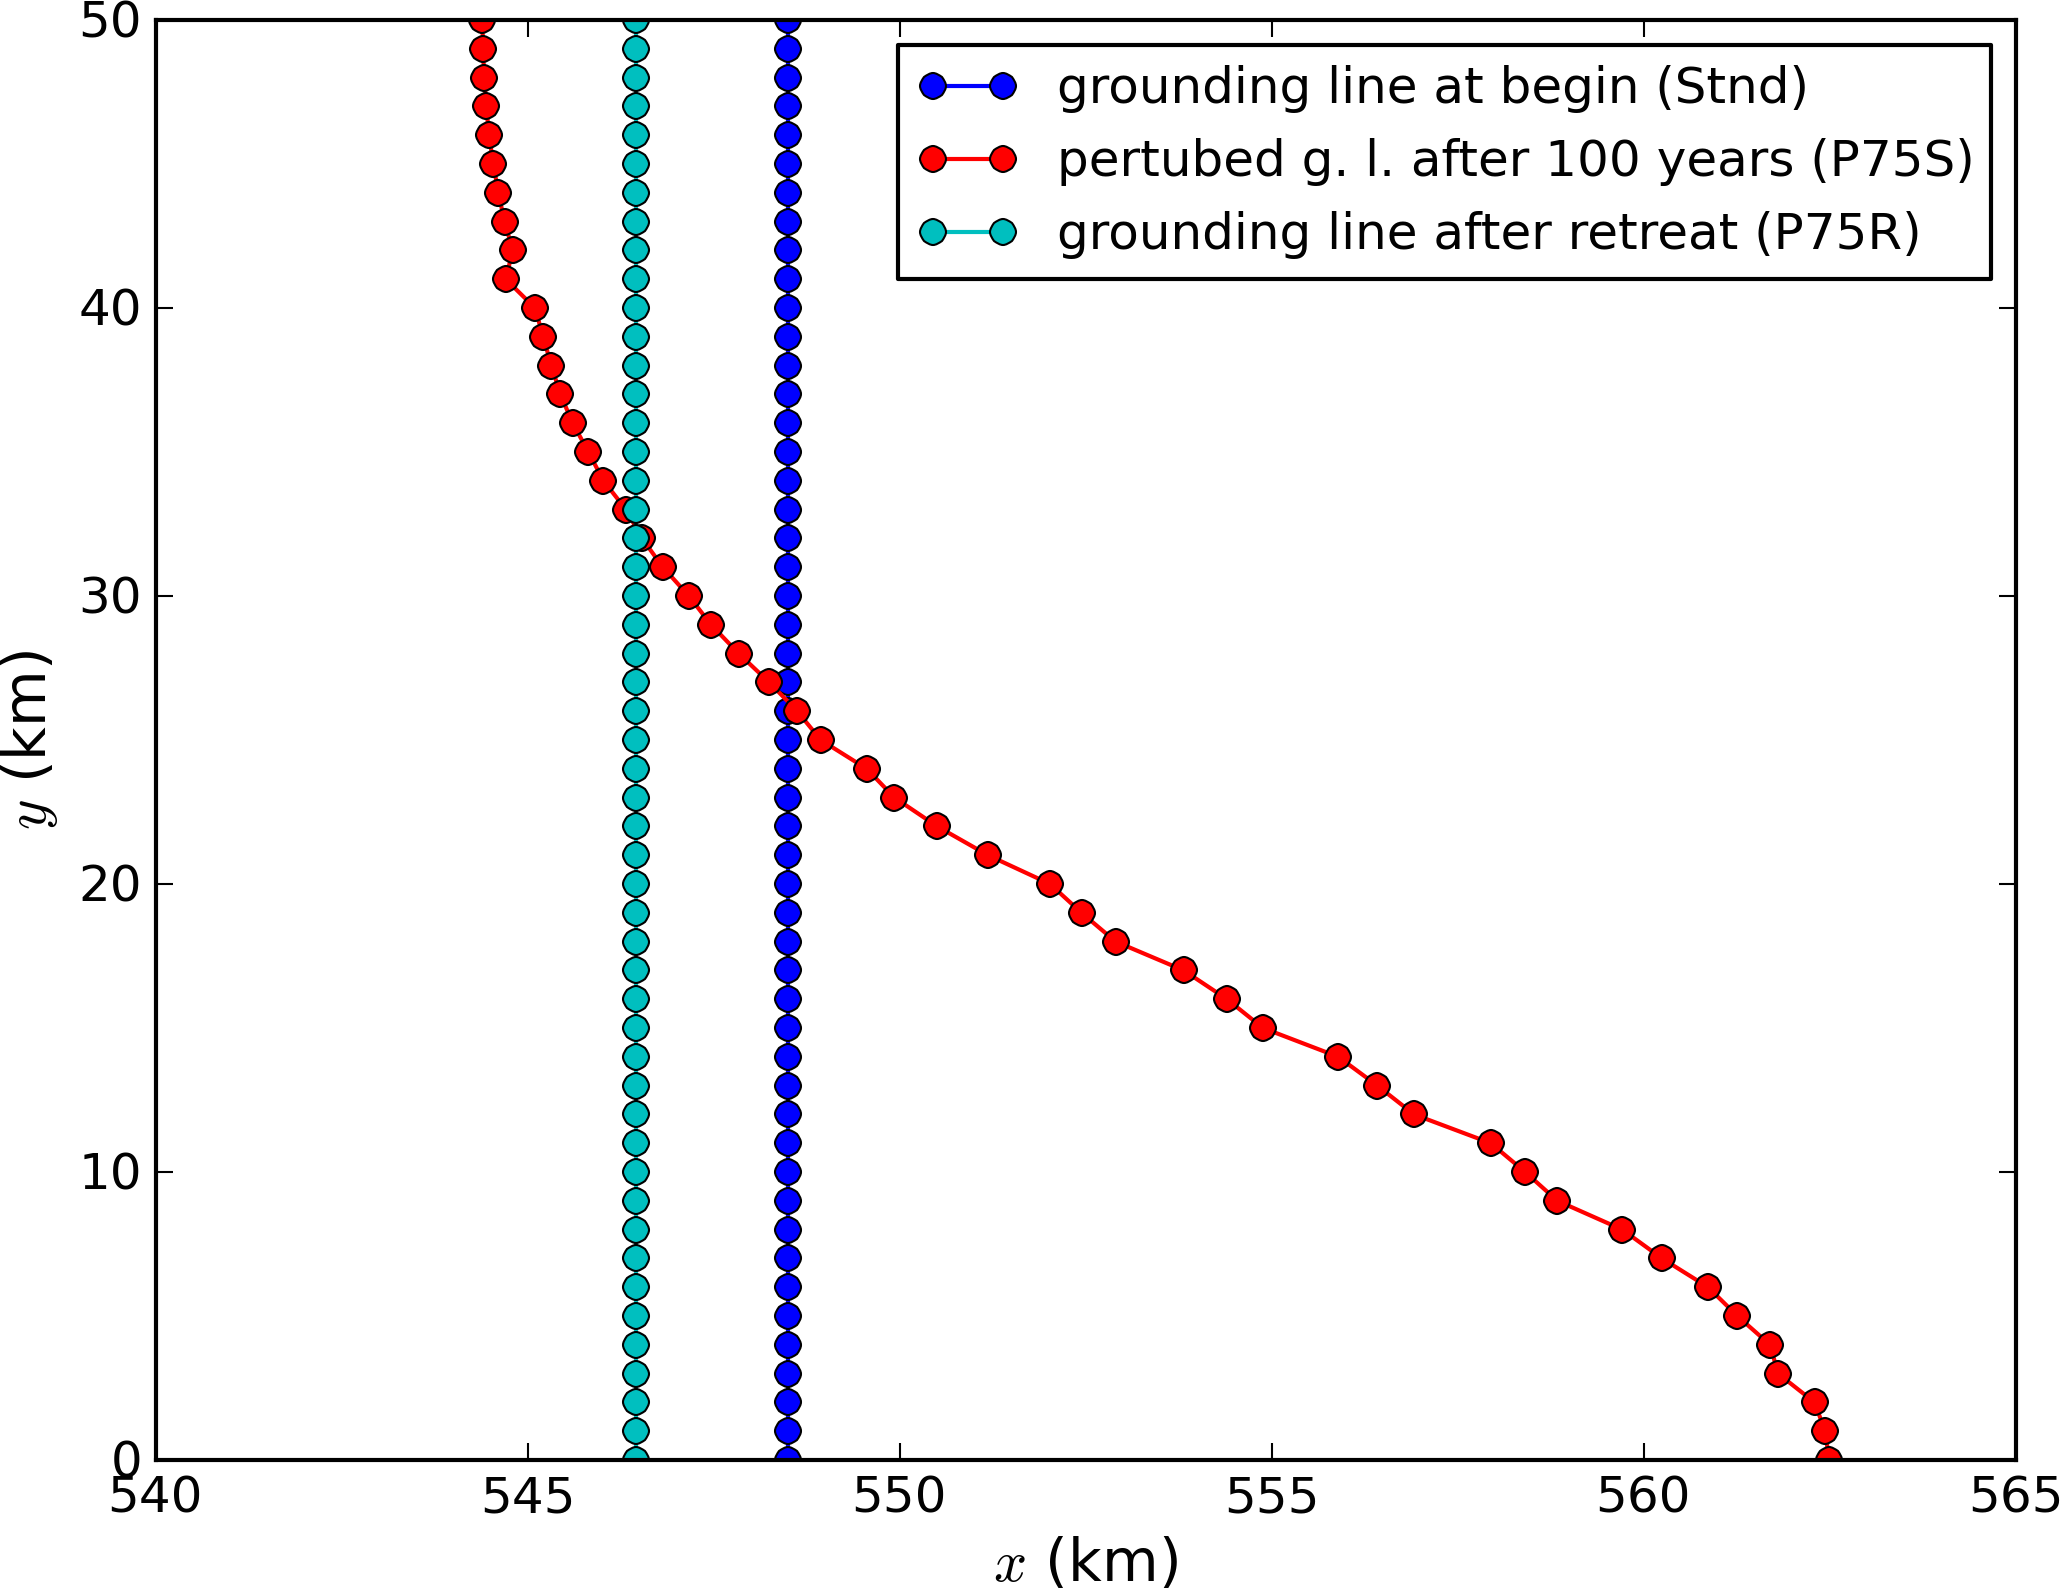
\includegraphics[width=3.3in,keepaspectratio=true]{Subgl}
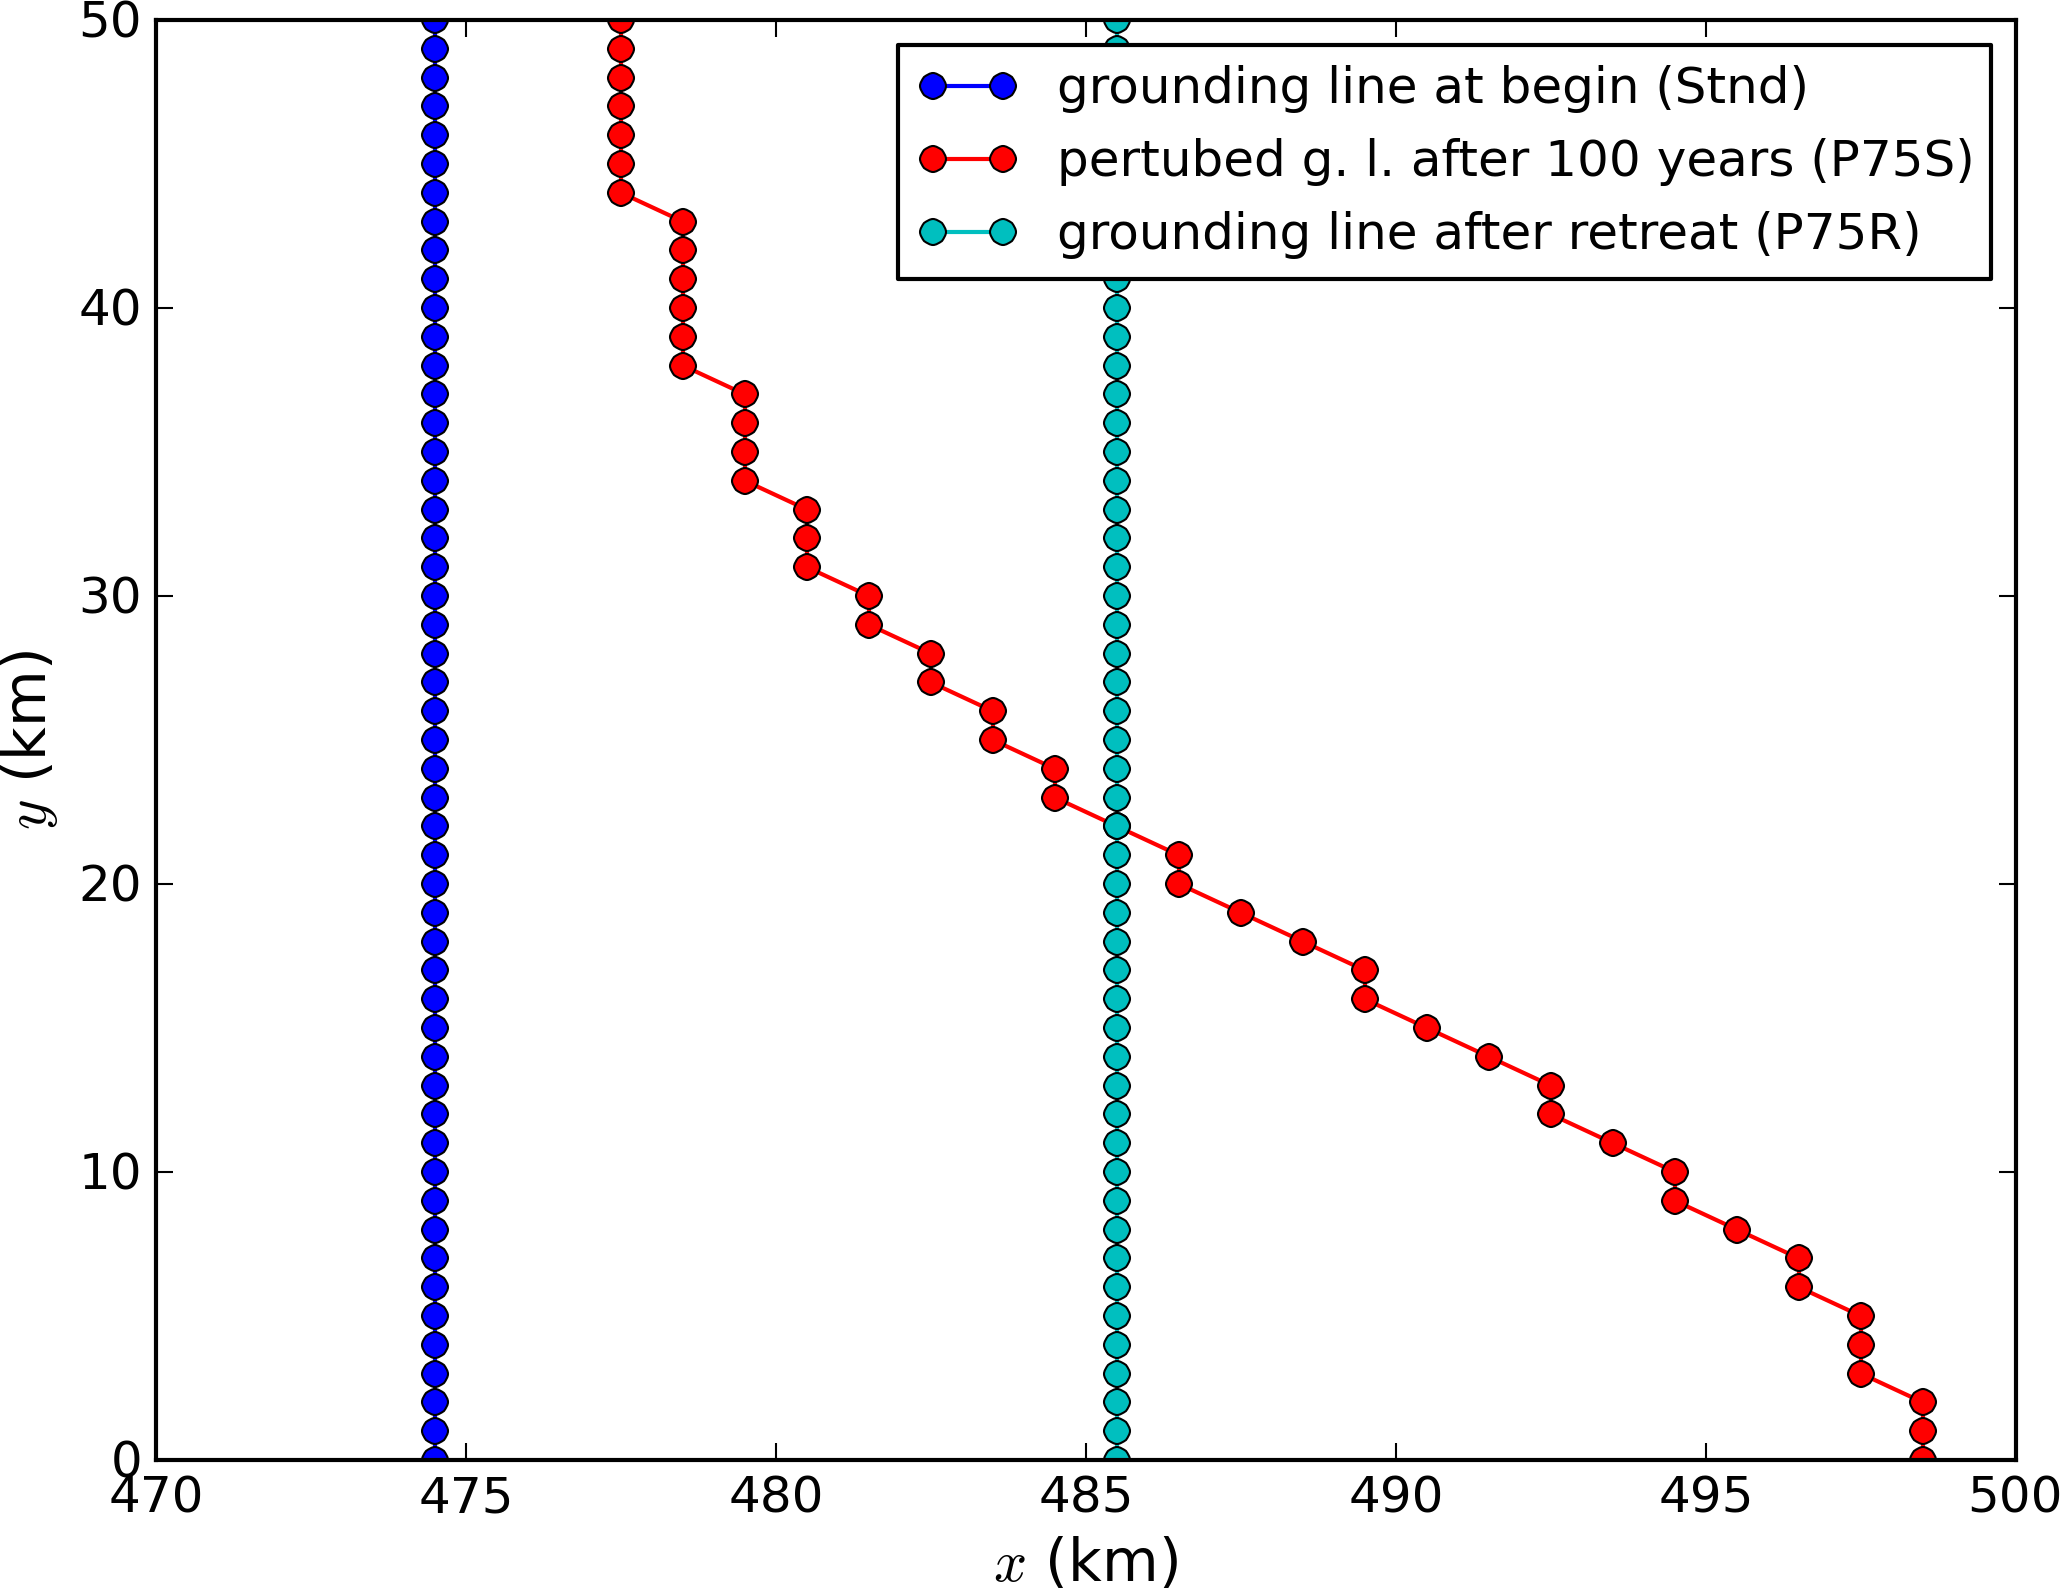
\includegraphics[width=3.3in,keepaspectratio=true]{NoSubgl}
\caption{Comparison between the grounding lines of the higher-amplitude (``\texttt{P75}'') MISMIP3d experiments performed with PISM when using the subgrid grounding line interpolation method (left) or not using it (right).  In both cases the SIA+SSA hybrid is used.}
\label{fig:Subgl}
\end{figure}

\begin{figure}[ht]
\centering
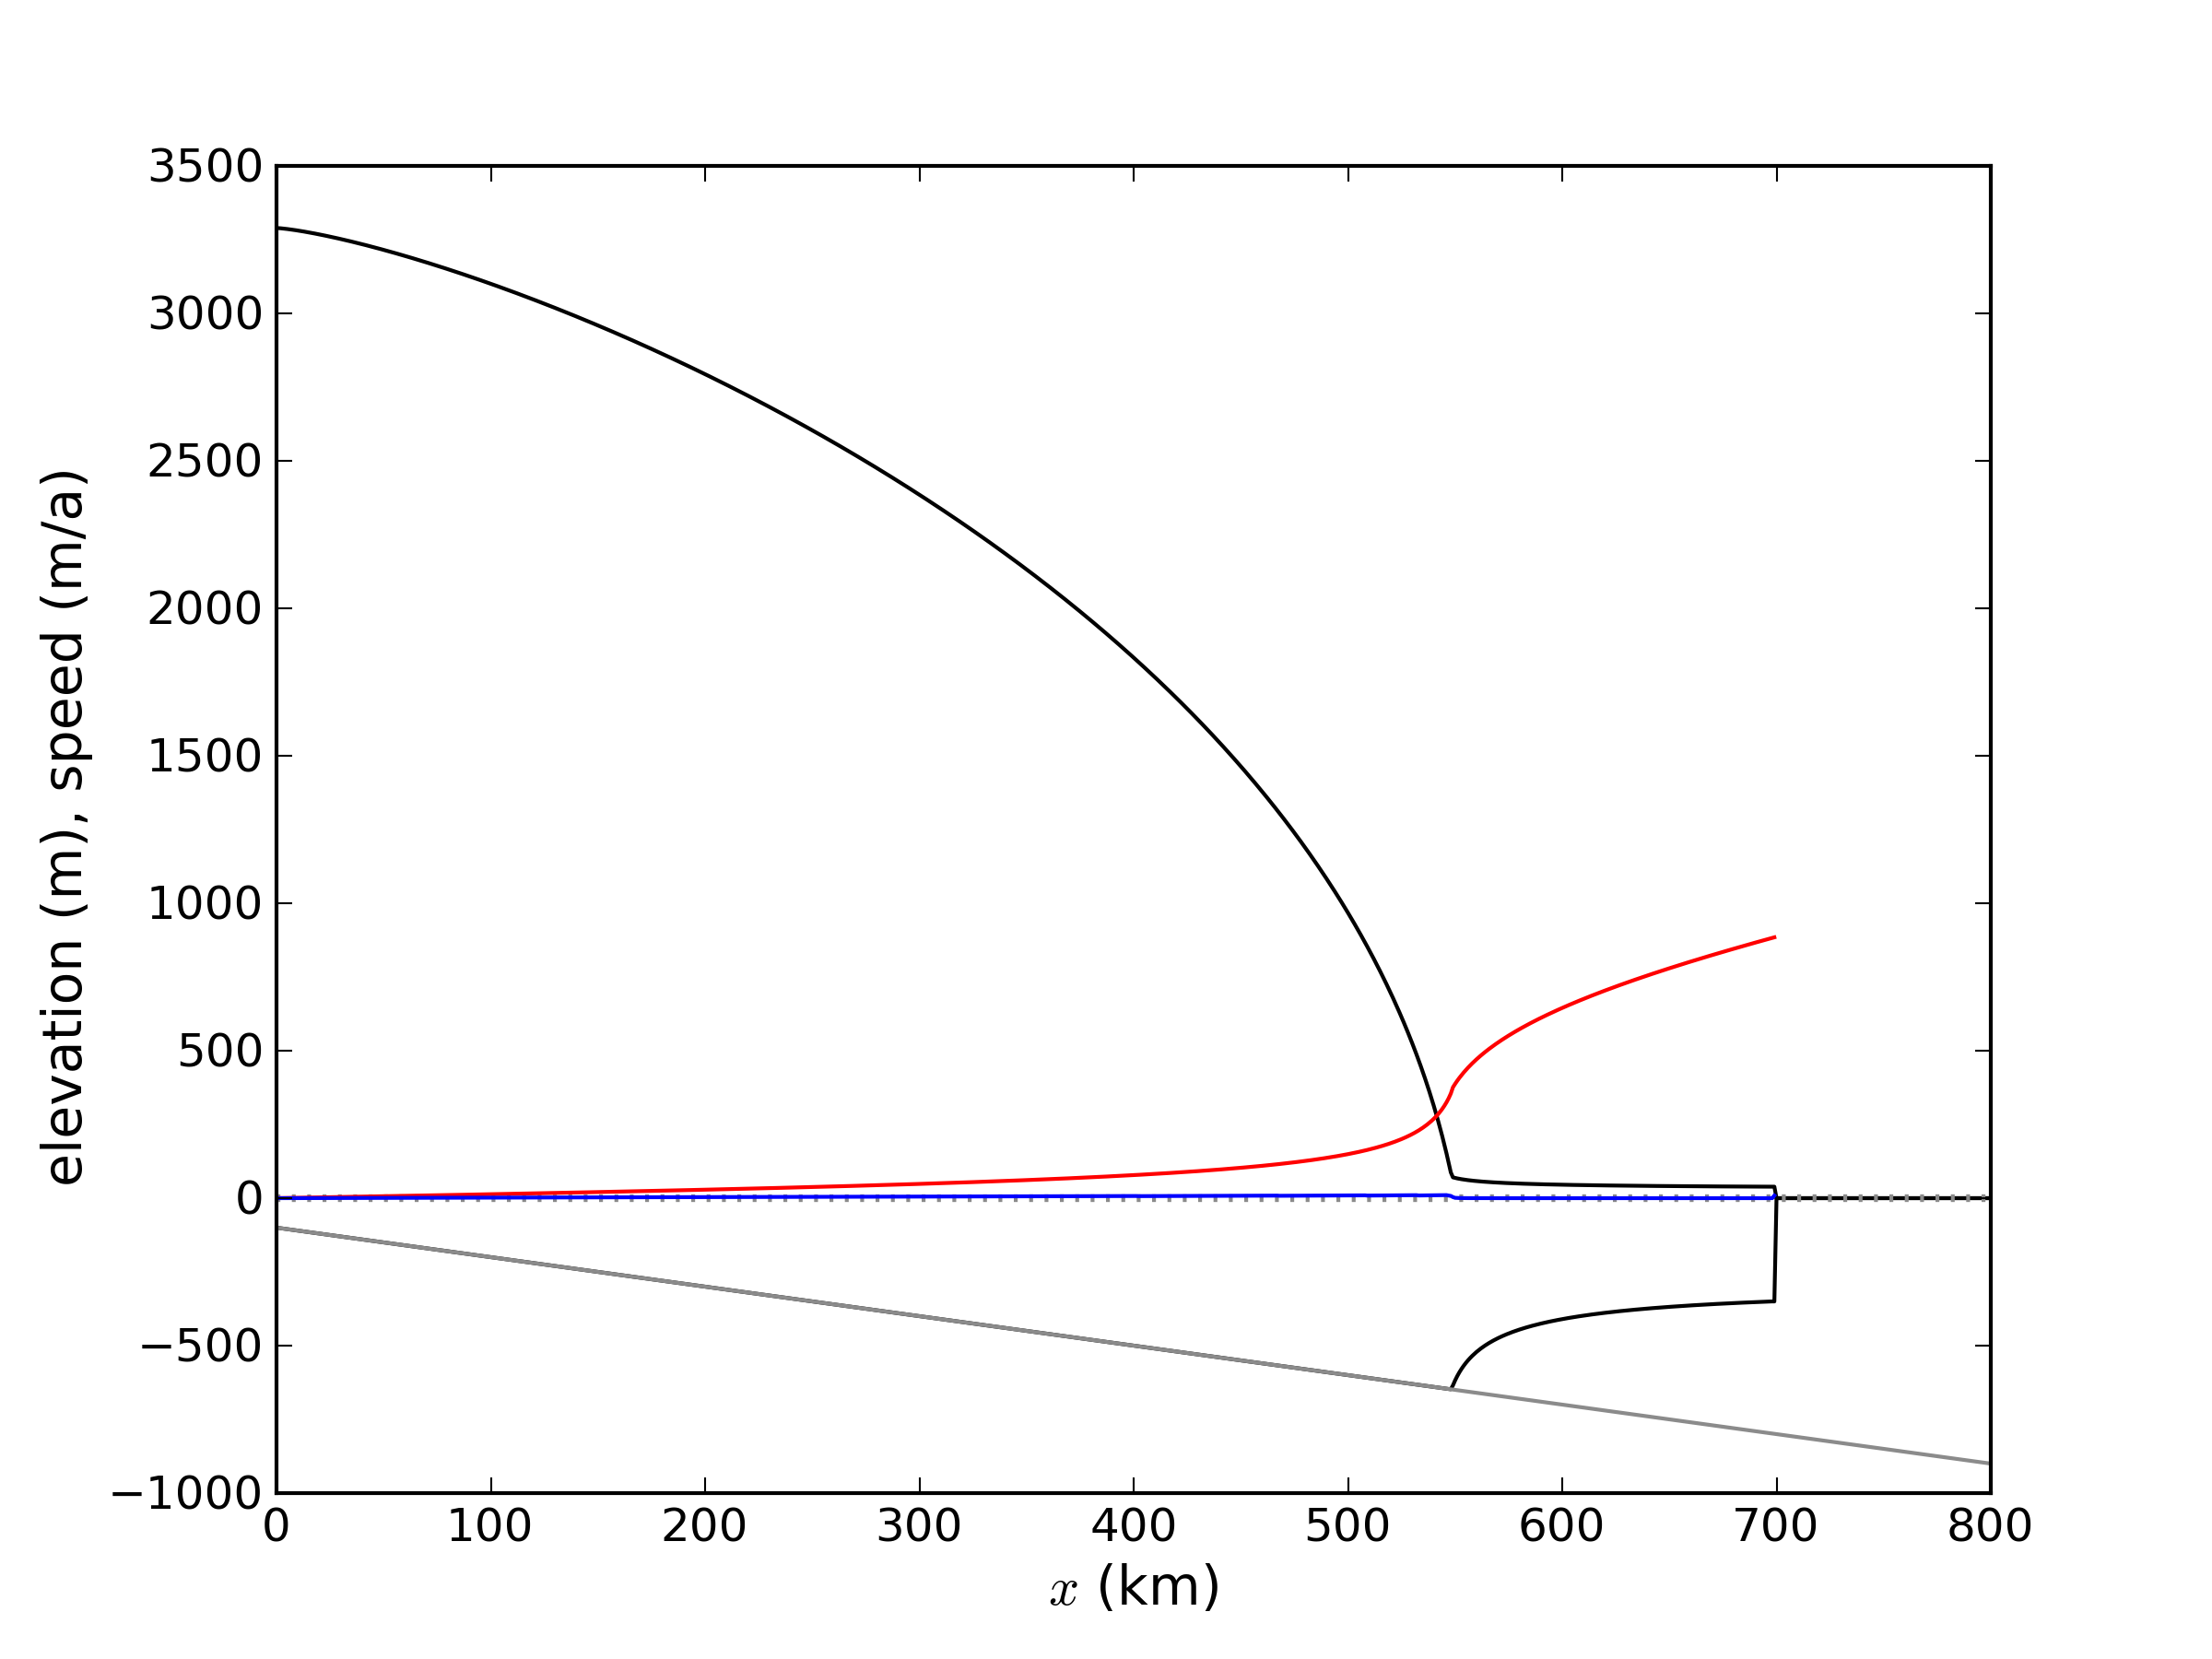
\includegraphics[width=5.0in,keepaspectratio=true]{comp-SIA-SSA}
\caption{The SIA velocities are negligible in the MISMIP3d standard experiment (``\texttt{Stnd}'').  The steady state ice geometry is plotted (black) together with the computed SSA velocity (red) and SIA velocity (blue). The SIA velocity reaches its maximum value of about $10\,$m/a at the grounding line, about two orders of magnitude less than the maximum of the SSA velocity.}
\label{fig:compSIASSA}
\end{figure}

%%% Local Variables: 
%%% mode: latex
%%% TeX-master: "manual"
%%% End: 
